% ------------------------------------------------------------------------------
% TYPO3 Version 10.0 - What's New (French Version)
%
% @author	Michael Schams <schams.net>
% @translator	Paul Blondiaux
% @reviewer	Pierrick Caillon
% @license	Creative Commons BY-NC-SA 3.0
% @link		http://typo3.org/download/release-notes/whats-new/
% @language	French
% ------------------------------------------------------------------------------

\section{Interface Utilisateur Backend}
\begin{frame}[fragile]
	\frametitle{Interface Utilisateur Backend}

	\begin{center}\huge{Chapitre 1~:}\end{center}
	\begin{center}\huge{\color{typo3darkgrey}\textbf{Interface Utilisateur Backend}}\end{center}

\end{frame}

% ------------------------------------------------------------------------------
% Feature | 56213 | Allow sorting file list by file meta data title

\begin{frame}[fragile]
	\frametitle{Interface Utilisateur Backend}
	\framesubtitle{Tri de la liste de fichiers}

	Les fichiers peuvent être triés par leur métadonnée «~titre~» depuis le contenu de type
	«~Liste de fichiers~».

	\begin{figure}
		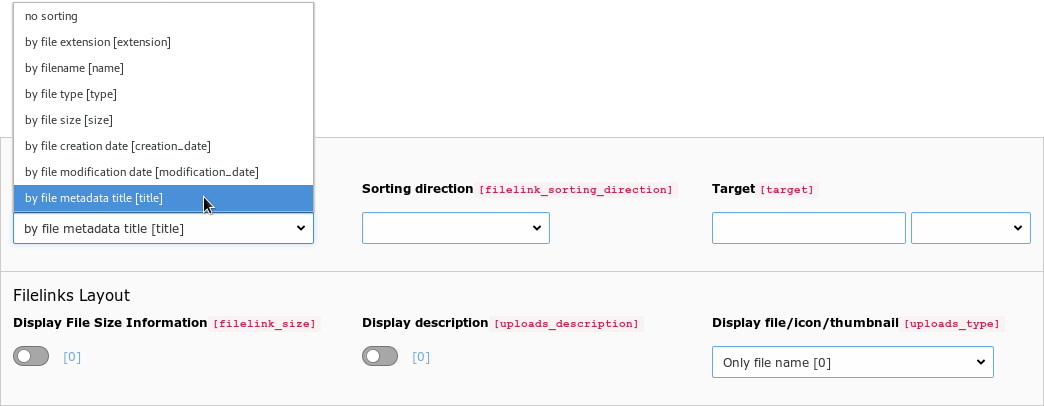
\includegraphics[width=0.90\linewidth]{BackendUserInterface/56213-FilelistSorting.png}
	\end{figure}

\end{frame}

% ------------------------------------------------------------------------------
% Feature | 85569 | Show scheduler information in the system information toolbar

\begin{frame}[fragile]
	\frametitle{Interface Utilisateur Backend}
	\framesubtitle{Barre d'informations système}

	La barre d'information système permet de consulter les informations liées au planificateur TYPO3.

	\begin{figure}
		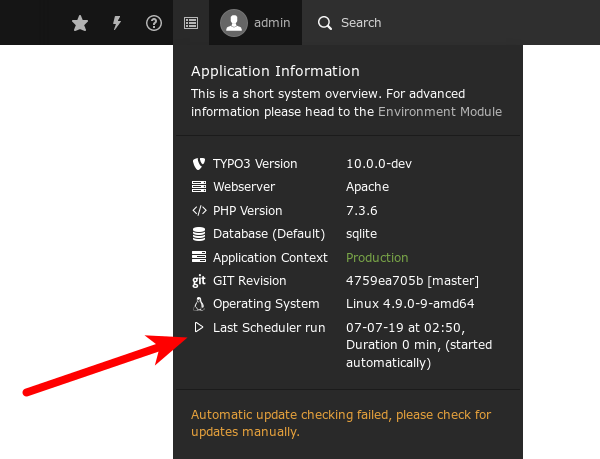
\includegraphics[width=0.50\linewidth]{BackendUserInterface/85569-SchedulerInfoInStatusBar.png}
	\end{figure}

\end{frame}

% ------------------------------------------------------------------------------
% Feature | 86629 | Implement LinkHandler for telephone numbers

\begin{frame}[fragile]
	\frametitle{Interface Utilisateur Backend}
	\framesubtitle{Gestionnaire de lien}

	Un nouveau gestionnaire de lien est ajouté et permet aux utilisateurs Backend de lier des numéros de
	téléphone grâce au protocole \texttt{tel:}.

	\begin{figure}
		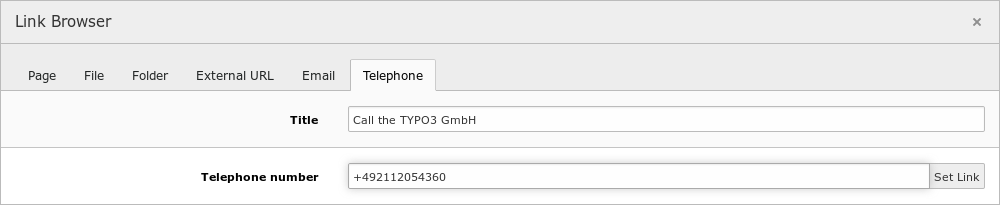
\includegraphics[width=0.90\linewidth]{BackendUserInterface/86629-TelephoneNumberLinkHandler.png}
	\end{figure}

	\begin{figure}
		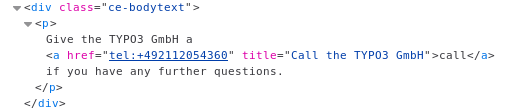
\includegraphics[width=0.60\linewidth]{BackendUserInterface/86629-TelephoneNumberLinkHandler2.png}
	\end{figure}

\end{frame}

% ------------------------------------------------------------------------------
% Feature | 87433 | Add changefreq and priority

\begin{frame}[fragile]
	\frametitle{Interface Utilisateur Backend}
	\framesubtitle{Sitemap SEO (1)}

	L'extension \texttt{EXT:seo} supporte les fréquences et priorités de mise à jour pour la Sitemap.
	Les propriétés de page (onglet «~SEO~») fournissent deux nouveaux champs.

	\begin{figure}
		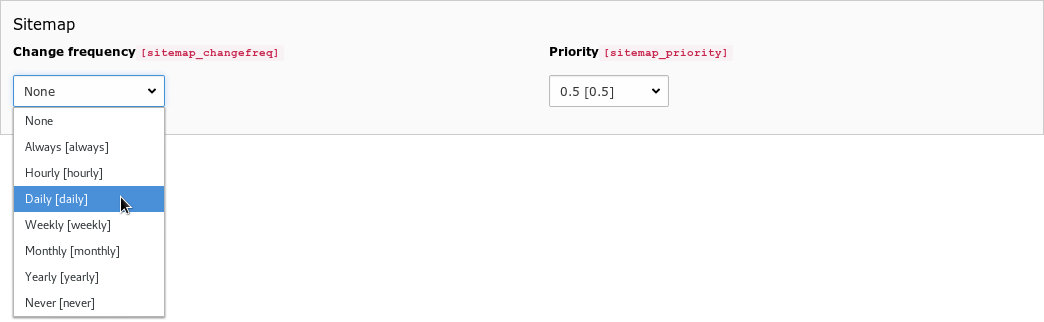
\includegraphics[width=0.90\linewidth]{BackendUserInterface/87433-SeoAddChangefreqAndPriority.png}
	\end{figure}

\end{frame}

% ------------------------------------------------------------------------------
% Feature | 87433 | Add changefreq and priority

\begin{frame}[fragile]
	\frametitle{Interface Backend}
	\framesubtitle{Sitemap SEO (2)}

	% decrease font size for code listing
	\lstset{basicstyle=\tiny\ttfamily}

	Ces paramètres peuvent aussi être définis en TypoScript, associés aux champs en base de données.
	
	\begin{lstlisting}
plugin.tx_seo {
  config {
    xmlSitemap {
      sitemaps {
        <unique key> {
          provider = TYPO3\CMS\Seo\XmlSitemap\RecordsXmlSitemapDataProvider
          config {
            ...
            changeFreqField = news_changefreq
            priorityField = news_priority
            ...
          }
        }
      }
    }
  }
}
	\end{lstlisting}

\end{frame}

% ------------------------------------------------------------------------------
% Feature | 84757 | Double click in structure tree changes label

\begin{frame}[fragile]
	\frametitle{Interface Utilisateur Backend}
	\framesubtitle{Formulaires}

	% decrease font size for code listing
	\lstset{basicstyle=\tiny\ttfamily}

	Les libellés des champs de formulaire sont éditables en double-cliquant directement sur le titre dans l'arborescence.

	\begin{figure}
		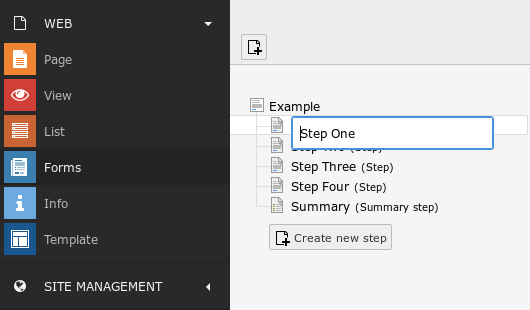
\includegraphics[width=0.60\linewidth]{ChangesForIntegrators/84757-DoubleClickToChangeLabel.png}
	\end{figure}

\end{frame}

% ------------------------------------------------------------------------------
